\documentclass[12pt]{article}
\usepackage{setspace}
\setstretch{1}
\usepackage{amsmath,amssymb, amsthm}
\usepackage{graphicx}
\usepackage{bm}
\usepackage[hang, flushmargin]{footmisc}
\usepackage[colorlinks=true]{hyperref}
\usepackage[nameinlink]{cleveref}
\usepackage{footnotebackref}
\usepackage{url}
\usepackage{listings}
\usepackage[most]{tcolorbox}
\usepackage{inconsolata}
\usepackage[papersize={8.5in,11in}, margin=1in]{geometry}
\usepackage{float}
\usepackage{caption}
\usepackage{esint}
\usepackage{url}
\usepackage{enumitem}
\usepackage{subfig}
\usepackage{wasysym}
\newcommand{\ilc}{\texttt}
\usepackage{etoolbox}
\usepackage{algorithm}
% \usepackage{algorithmic}
\usepackage[noend]{algpseudocode}
\usepackage{tikz}
\usepackage{listings}
\usepackage{color}
\usetikzlibrary{matrix,positioning,arrows.meta,arrows}
\patchcmd{\thebibliography}{\section*{\refname}}{}{}{}



\definecolor{dkgreen}{rgb}{0,0.6,0}
\definecolor{gray}{rgb}{0.5,0.5,0.5}
\definecolor{mauve}{rgb}{0.58,0,0.82}

\lstset{frame=tb,
  language=Python,
  aboveskip=3mm,
  belowskip=3mm,
  showstringspaces=false,
  columns=flexible,
  basicstyle={\small\ttfamily},
  numbers=none,
  numberstyle=\tiny\color{gray},
  keywordstyle=\color{blue},
  commentstyle=\color{dkgreen},
  stringstyle=\color{mauve},
  breaklines=true,
  breakatwhitespace=true,
  tabsize=3
}

\begin{document}

\title{\textbf{CSDS 313: Assignment 2}}

\author{Shaochen (Henry) ZHONG, \ilc{sxz517} \\Ningjia HUANG, \ilc{nsh239}}
\date{Due and submitted on 10/19/2020 \\ Issued by Dr. Koyut{\"u}rk}
\maketitle



\section*{Problem 1}
\subsection*{(a)}
Mean of Uniform Distribution = $\frac{a + b}{2} = \mu$ \\
Standard Deviation of Uniform Distribution = $\sqrt{\frac{(b-a)^2}{12}} = \frac{b-a}{2\sqrt{3}} = \sigma$ \\
\begin{center}
    $a + b = 2\mu$ \\
    $b - a = 2\sqrt{3} \sigma$ \\
    $\Rightarrow b = \mu + \sqrt{3} \sigma$ \\
    $\Rightarrow a = \mu - \sqrt{3} \sigma$
\end{center}
Plugging in $\mu = 2$ and $\sigma = 5$ into $a$ and $b$, we get:
\begin{center}
    $a = 2 - 5\sqrt{3}$\\
    $b = 2 + 5\sqrt{3}$
\end{center}

\subsection*{(b)}
25th percentile of normal distribution $= \Phi^{-1}(0.25,\mu,\sigma)$\\
75th percentile of normal distribution $= \Phi^{-1}(0.75,\mu,\sigma)$\\
25th percentile of uniform distribution $\Rightarrow 0.25 = \frac{x_{25}-a}{b-a} \Rightarrow x_{25} = 0.25b + 0.75a$
75th percentile of uniform distribution $\Rightarrow 0.75 = \frac{x_{75} - a}{b-a} \Rightarrow x_{75} = 0.75b + 0.25a$
$0.25b + 0.75a = \Phi^{-1}(0.25,\mu,\sigma)$\\
$0.75b + 0.25a = \Phi^{-1}(0.75,\mu,\sigma)$\\
$\Rightarrow a = \frac{3\Phi^{-1}(0.25,\mu,\sigma-\Phi^{-1}(0.75,\mu,\sigma))}{2}$\\
$\Rightarrow b = \frac{3\Phi^{-1}(0.75,\mu,\sigma)-\Phi^{-1}(0.25,\mu,\sigma)}{2}$\\
Plugging in $\mu = 2$ and $\sigma = 5$ into $a$ and $b$ and using the following code:
\begin{lstlisting}
    def calc_percentile():
        print(norm.ppf(0.25,2,5))
        print(norm.ppf(0.75,2,5))
\end{lstlisting}
We get the values for $a$ and $b$:
\begin{center}
    $a = -1.3724$ \\
    $b = 5.3724$
\end{center}

\subsection*{Plots and Analysis}

\begin{figure}[H]
    \centering
    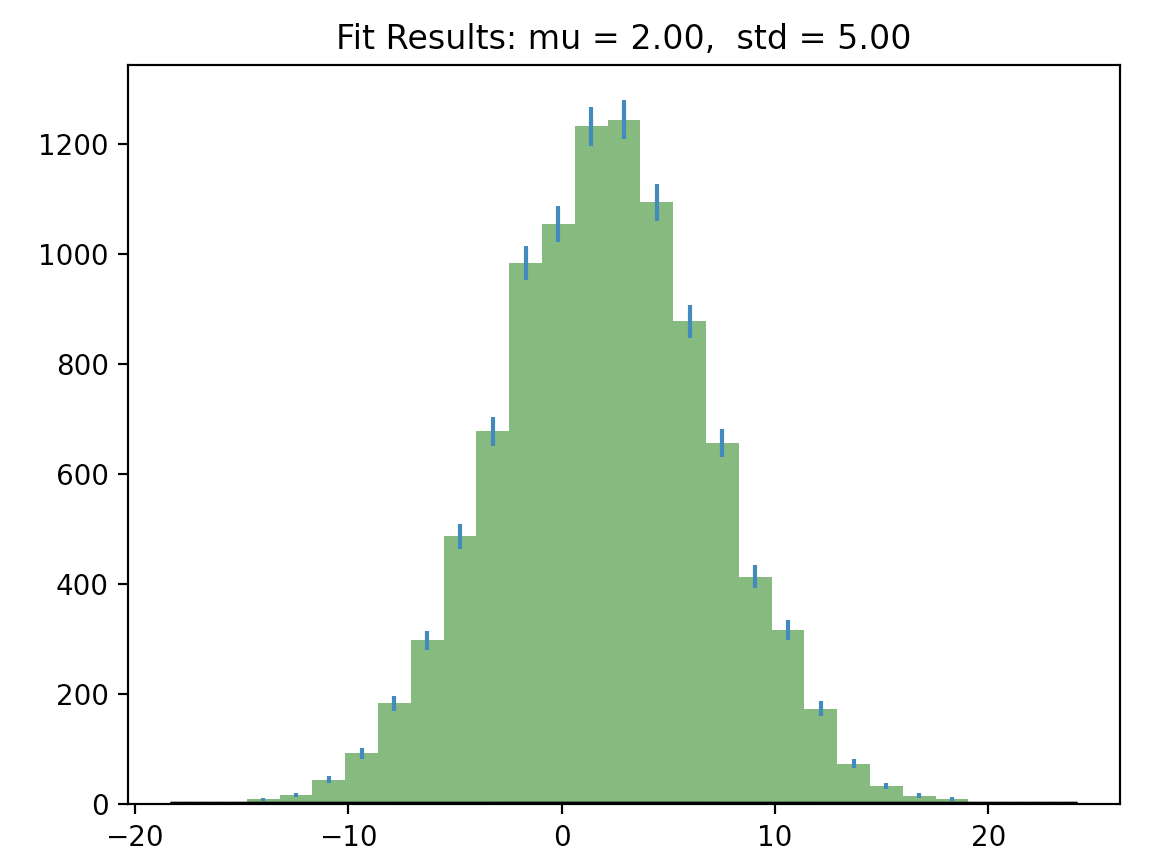
\includegraphics[scale=0.3]{{fig/normal_hist.png}}
    \caption{Normal Distribution Histogram with Error Bars}
\end{figure}

\begin{lstlisting}
    np.random.seed(1)
    sample = norm.rvs(loc=2, scale=5, size=10000)
    n, bins, _ = plt.hist(sample,bins=25,density=False,alpha=0.6,color='g')
    mid = 0.5*(bins[1:] + bins[:-1])
    plt.errorbar(mid, n, yerr=np.sqrt(n), fmt='none')
    xmin, xmax = plt.xlim()
    x = np.linspace(xmin, xmax, 100)
    p = norm.pdf(x, 2, 5)
    plt.plot(x, p, 'k', linewidth=2)
    title = "Fit Results: mu = %.2f,  std = %.2f" % (2, 5)
    plt.title(title)
    plt.show()
\end{lstlisting}

\begin{figure}[H]
    \centering
    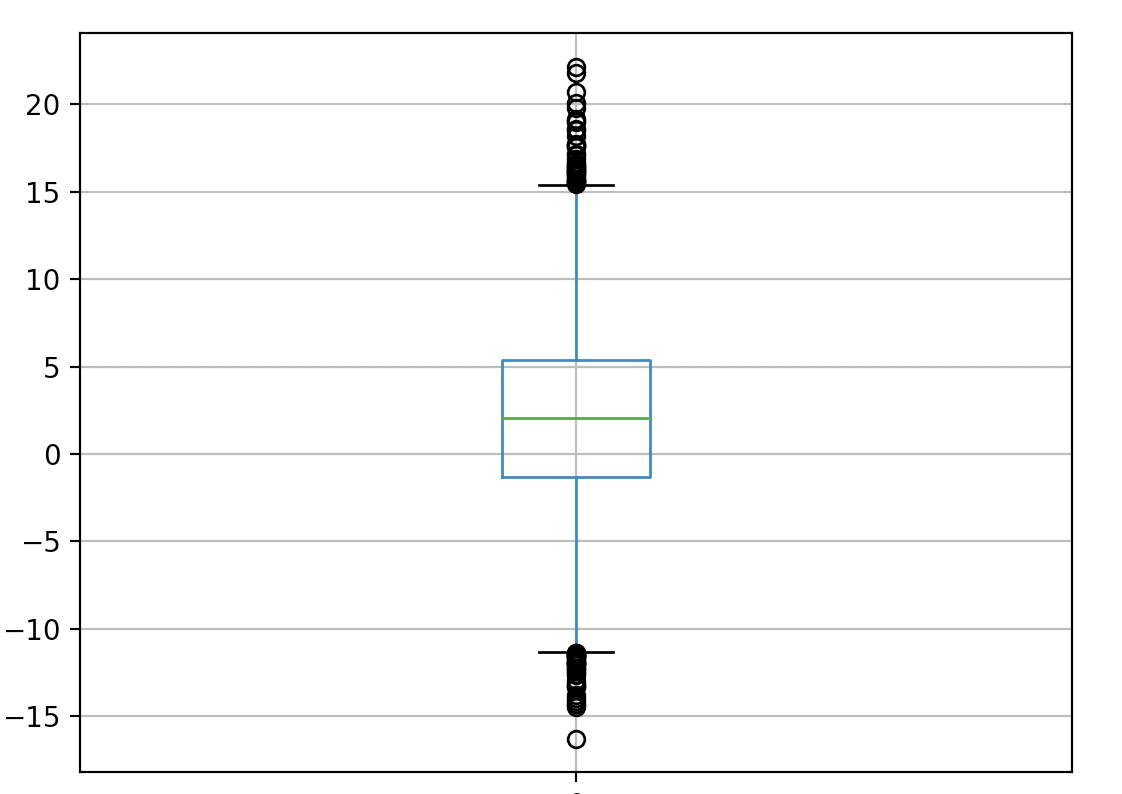
\includegraphics[scale=0.3]{{fig/normal_box.png}}
    \caption{Normal Distribution Boxplot}

\end{figure}
\begin{lstlisting}
    np.random.seed(1)
    sample = norm.rvs(loc=2, scale=5, size=10000)
    df = pd.DataFrame(sample)
    df.boxplot()
    plt.show()
\end{lstlisting}

\begin{figure}[H]
    \centering
    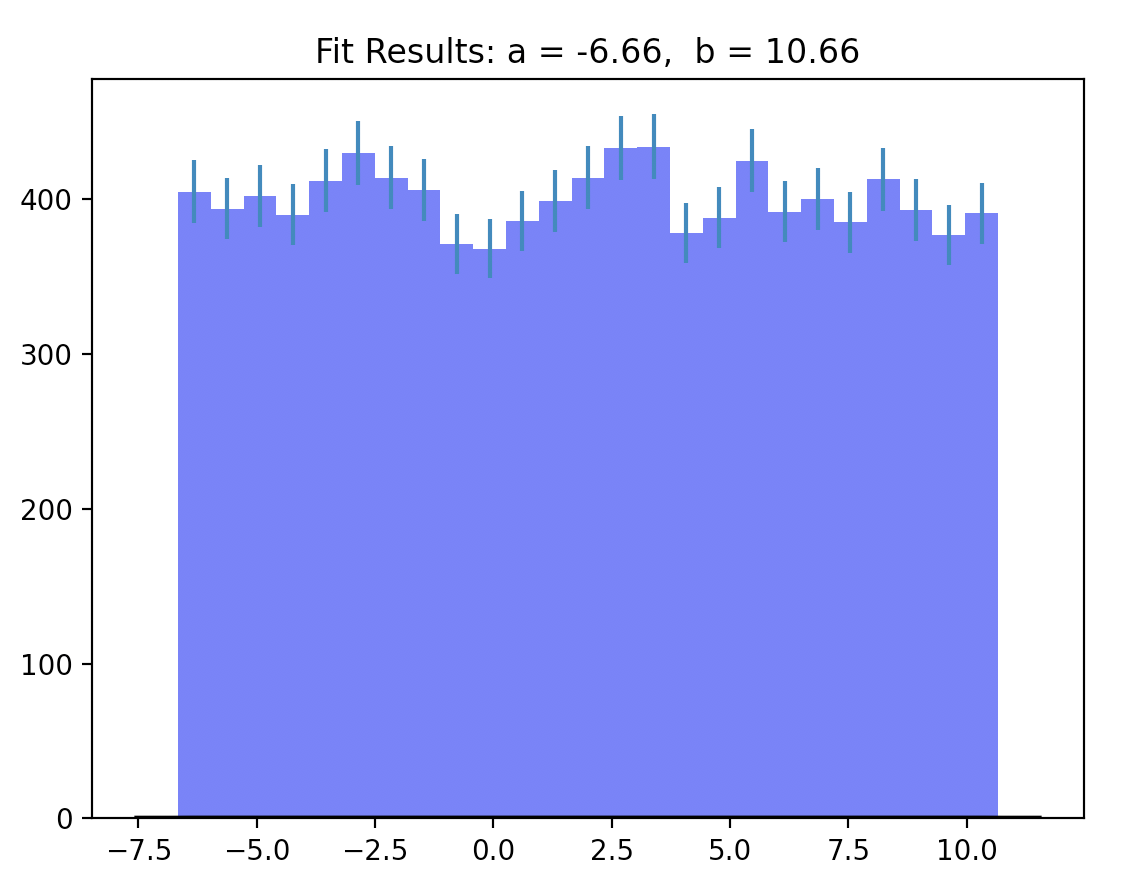
\includegraphics[scale=0.3]{{fig/u1_hist.png}}
    \caption{Uniform Distribution 1 Histogram with Error Bars}

\end{figure}
\begin{lstlisting}
    np.random.seed(1)
    sample = uniform.rvs(loc=2-5*math.sqrt(3), scale=10*math.sqrt(3), size=10000)
    n, bins, _ = plt.hist(sample,bins=25,density=False,alpha=0.6,color='b')
    mid = 0.5*(bins[1:] + bins[:-1])
    plt.errorbar(mid, n, yerr=np.sqrt(n), fmt='none')
    xmin, xmax = plt.xlim()
    x = np.linspace(xmin, xmax, 50)
    p = uniform.pdf(x, 2-5*math.sqrt(3), 10*math.sqrt(3))
    plt.plot(x, p, 'k', linewidth=2)
    title = "Fit Results: a = %.2f,  b = %.2f" % (2-5*math.sqrt(3), 2+5*math.sqrt(3))
    plt.title(title)
    plt.show()
\end{lstlisting}

\begin{figure}[H]
    \centering
    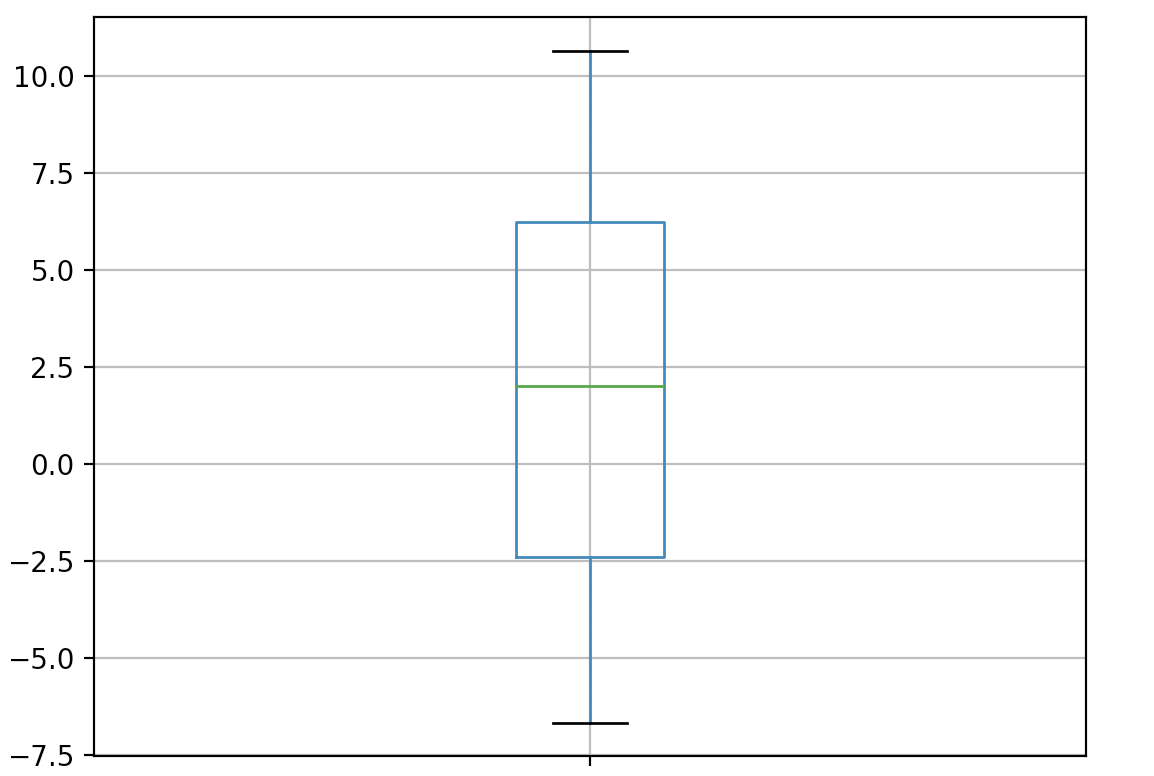
\includegraphics[scale=0.3]{{fig/u1_boxplot.png}}
    \caption{Uniform Distribution 1 Boxplot}

\end{figure}
\begin{lstlisting}
    np.random.seed(1)
    sample = uniform.rvs(loc=2-5*math.sqrt(3), scale=10*math.sqrt(3), size=10000)
    df = pd.DataFrame(sample)
    df.boxplot()
    plt.show()
\end{lstlisting}

\begin{figure}[H]
    \centering
    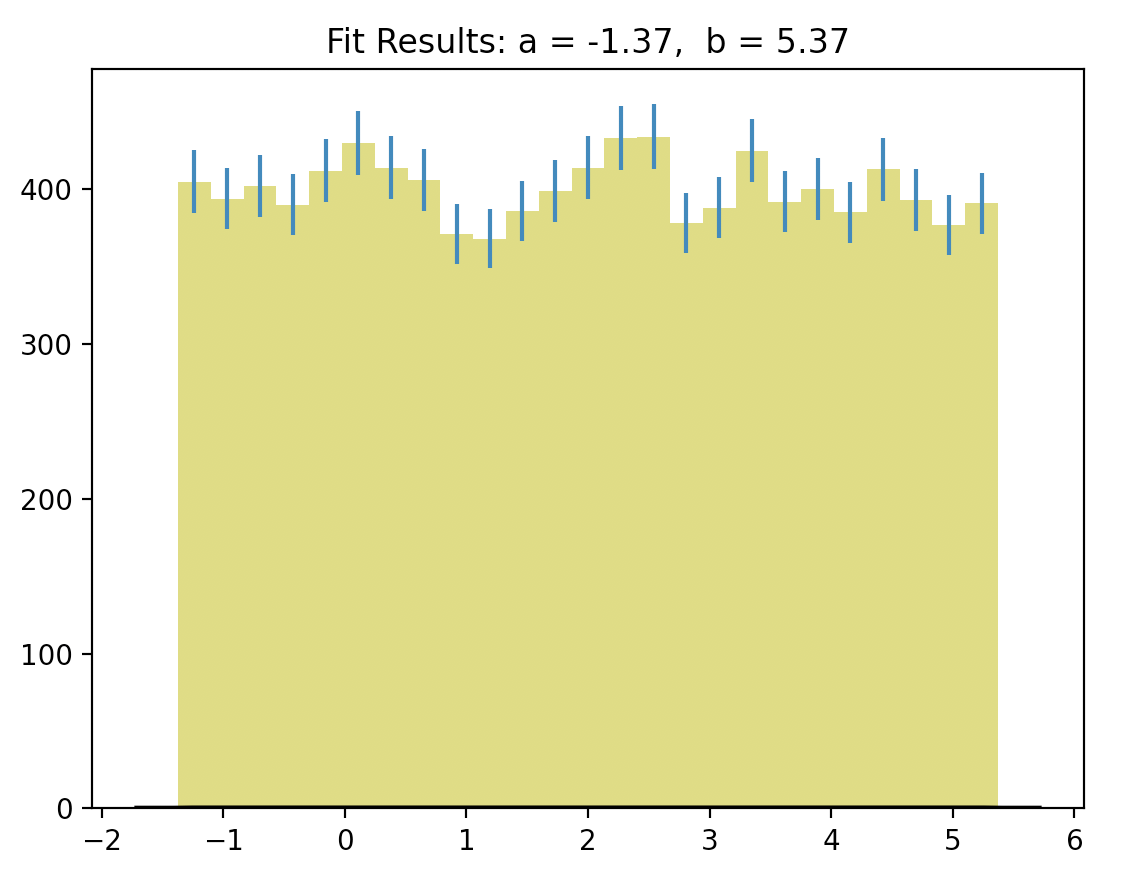
\includegraphics[scale=0.3]{{fig/u2_hist.png}}
    \caption{Uniform Distribution 2 Histogram with Error Bars}

\end{figure}
\begin{lstlisting}
    np.random.seed(1)
    sample = uniform.rvs(loc=-1.3724, scale=6.7448, size=10000)
    n, bins, _ = plt.hist(sample,bins=25,density=False,alpha=0.6,color='y')
    mid = 0.5*(bins[1:] + bins[:-1])
    plt.errorbar(mid, n, yerr=np.sqrt(n), fmt='none')
    xmin, xmax = plt.xlim()
    x = np.linspace(xmin, xmax, 50)
    p = uniform.pdf(x, -1.3723, 6.7448)
    plt.plot(x, p, 'k', linewidth=2)
    title = "Fit Results: a = %.2f,  b = %.2f" % (-1.3724, 5.3724)
    plt.title(title)
    plt.show()
\end{lstlisting}

\begin{figure}[H]
    \centering
    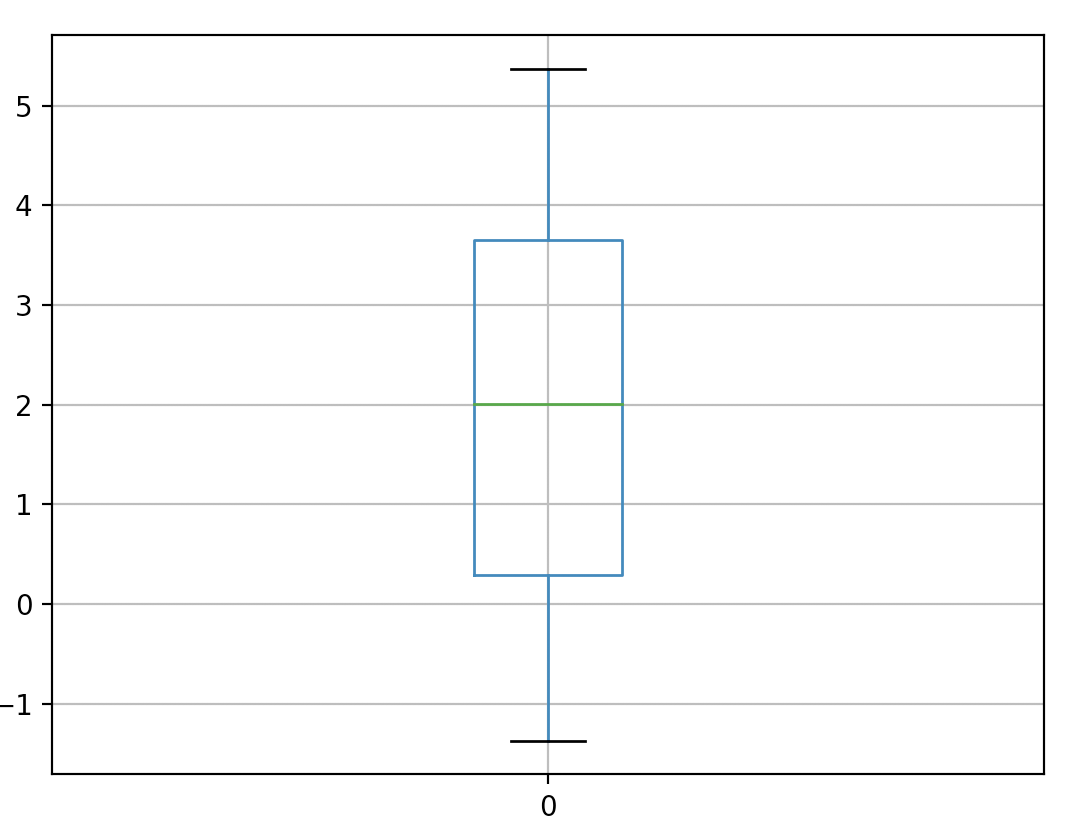
\includegraphics[scale=0.3]{{fig/u2_box.png}}
    \caption{Uniform Distribution 2 Boxplot}

\end{figure}
\begin{lstlisting}
    np.random.seed(1)
    sample = uniform.rvs(loc=-1.3724, scale=6.7448, size=10000)
    df = pd.DataFrame(sample)
    df.boxplot()
    plt.show()
\end{lstlisting}

\noindent The histograms of uniform distribution 1 and 2 are quite different from the histogram of normal distribution. For uniform distribution
1 and 2, the $10,000$ sample points are more evenly distributed in the range comparing with normal distribution. For normal distribution,
we can tell around $2,500$ sample points lie in the range $[0,6]$. A few points start appearing around $-18$, then more appear until they
reach the threshold(around 6), then the number decreases again. From the boxplots, we can tell the range of the points are larger for normal
distribution than for uniform distributions. Also, for normal distribution, the distance between the minimum to the 25 percentile(around 10)
is much larger than the distance between minimum and 25 percentile for uniform distributions(around 5.5 and 1.5). This is understandable because
for uniform distributions, all points are equally likely to distribute in a certain range. However, for normal distribution, few points are distributed at the beginning
and then the number of points increases gradually. Therefore, it takes longer time to reach the 25 percentile. \\
The shapes of these two uniform distributions are similar since for both of them, points are evenly distributed in the range. However, the range of the first
uniform distribution is much larger than the second uniform distribution.

\section*{Problem 2: }
\subsection*{(a)}
\subsubsection*{airport: }
\begin{lstlisting}
    df = pd.read_csv("airport_routes.csv")
    array = df['NumberOfRoutes'].to_numpy()
    sum = 0
    for i in array:
        sum += np.log(i)
    alpha = 1 + 3409 * sum**(-1)
\end{lstlisting}
Therefore, $\alpha = 1.612091630402382$.
\begin{figure}[H]
    \centering
    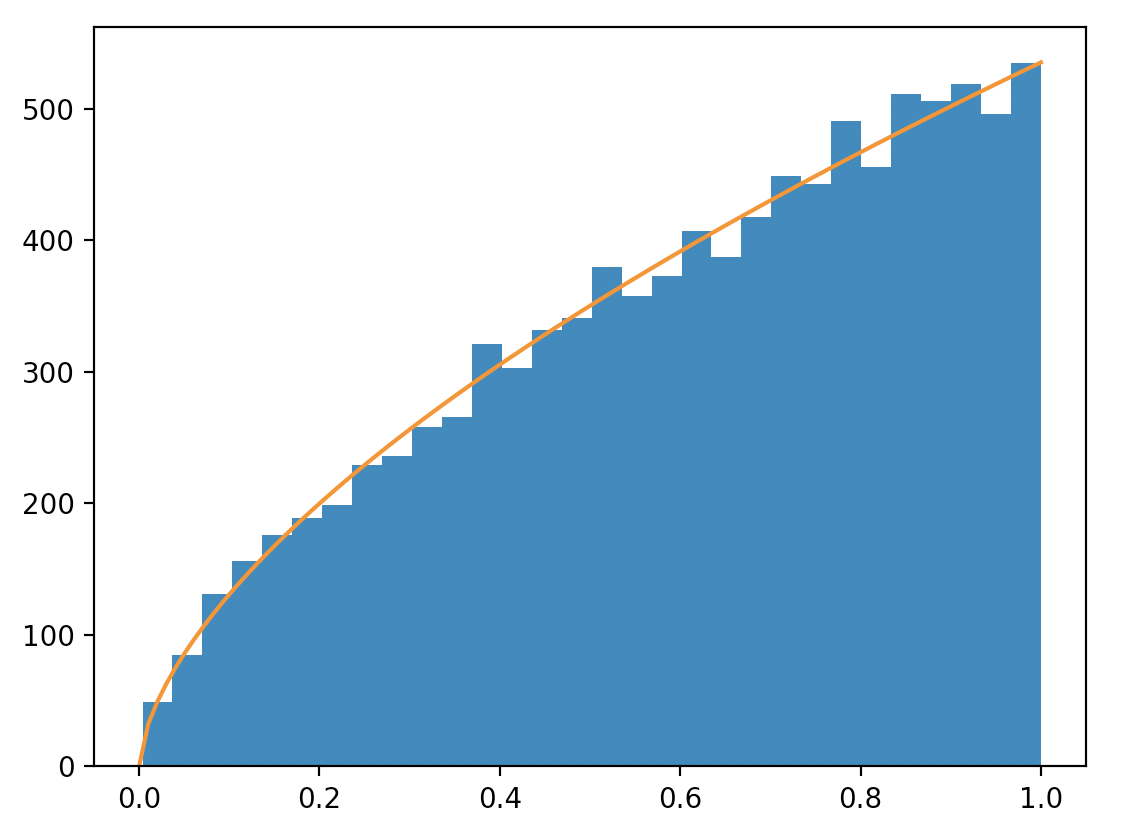
\includegraphics[scale=0.3]{{fig/power_air.png}}
    \caption{Power Law Distribution for Airport Routes}
\end{figure}

\subsubsection*{movie: }
\begin{lstlisting}
    df = pd.read_csv("movie_votes.csv")
    array = df['AverageVote'].to_numpy()
    sum = 0
    for i in array:
        sum += np.log(i/1.9)
    alpha = 1 + 4392 * sum**(-1)
\end{lstlisting}
Therefore, $\alpha = 1.8505152700921788$.
\begin{figure}[H]
    \centering
    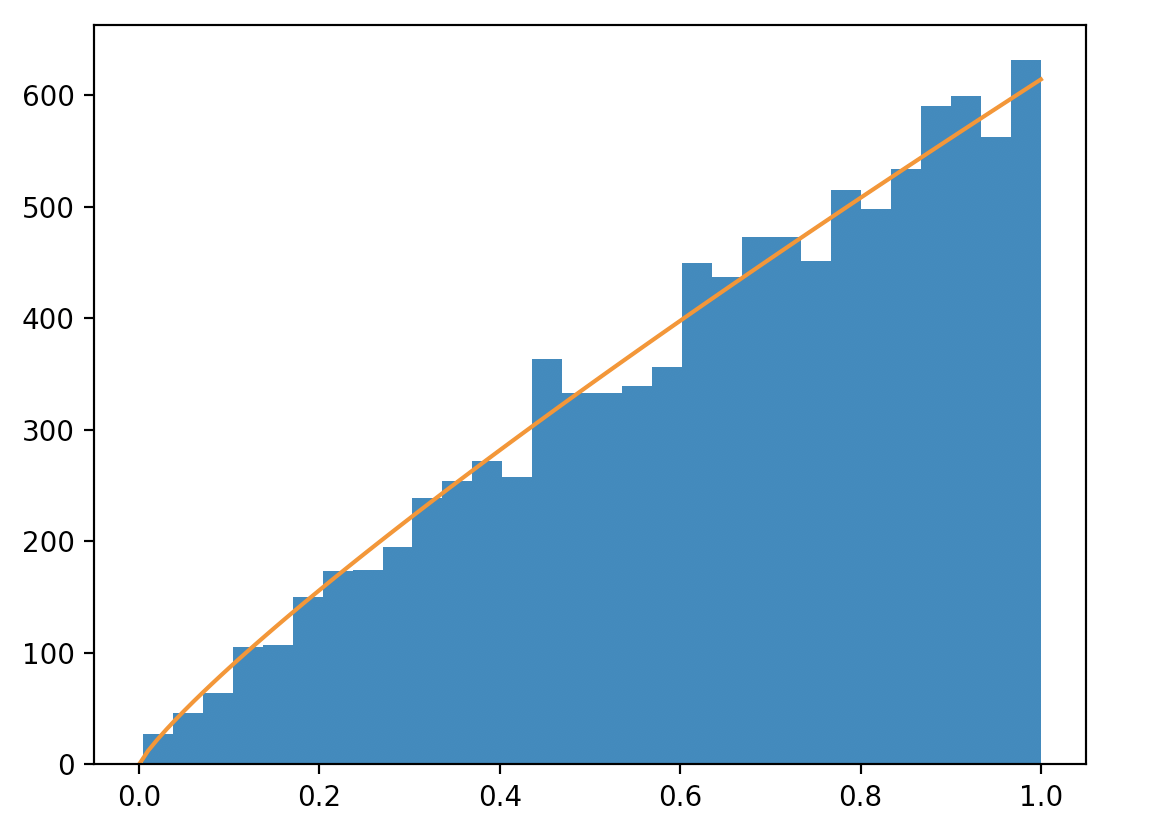
\includegraphics[scale=0.3]{{fig/power_movie.png}}
    \caption{Power Law Distribution for Movie Votes}
\end{figure}

\subsection*{(b)}
\subsubsection*{airport: }
\begin{lstlisting}
    df = pd.read_csv("airport_routes.csv")
    print(1/df.mean())
\end{lstlisting}
Therefore, $\lambda = 0.05039$.
\begin{figure}[H]
    \centering
    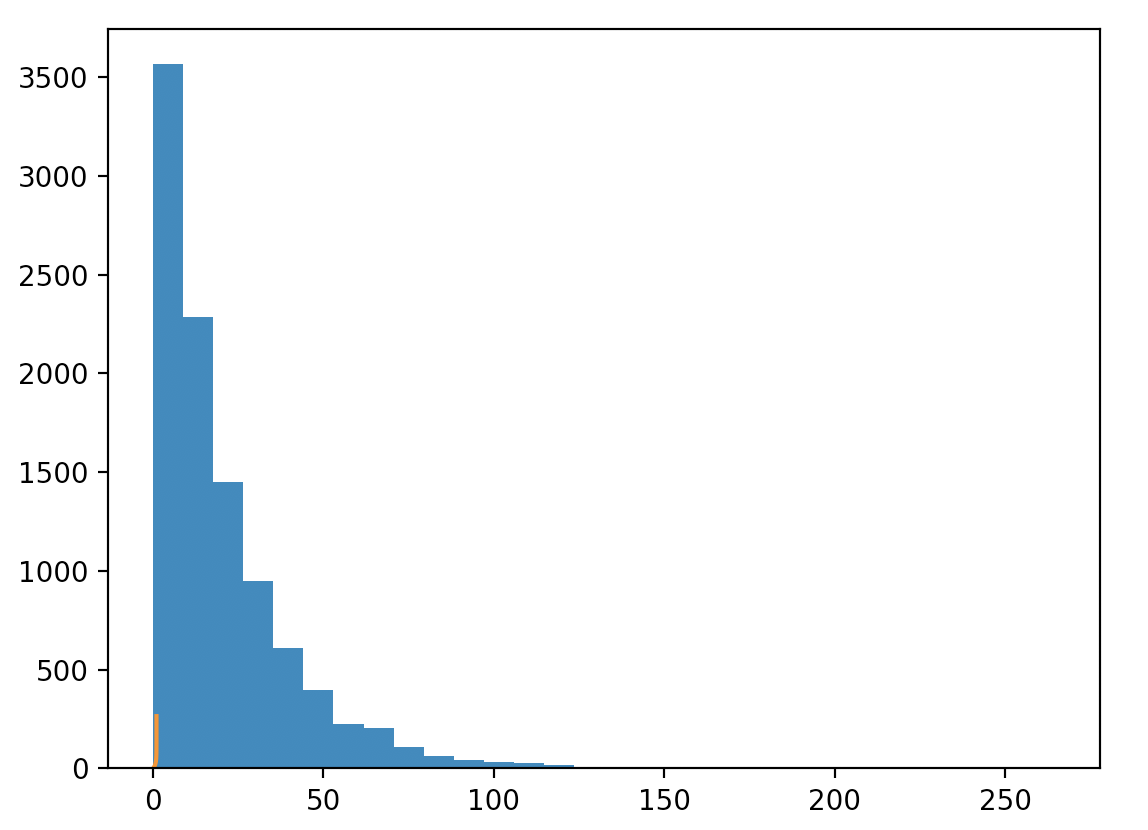
\includegraphics[scale=0.3]{{fig/exp_air.png}}
    \caption{Exponential Distribution for Airport Routes}
\end{figure}

\subsubsection*{movie: }
\begin{lstlisting}
    df = pd.read_csv("movie_votes.csv")
    print(1/df.mean())
\end{lstlisting}
Therefore, $\lambda = 0.160593$.

\begin{figure}[H]
    \centering
    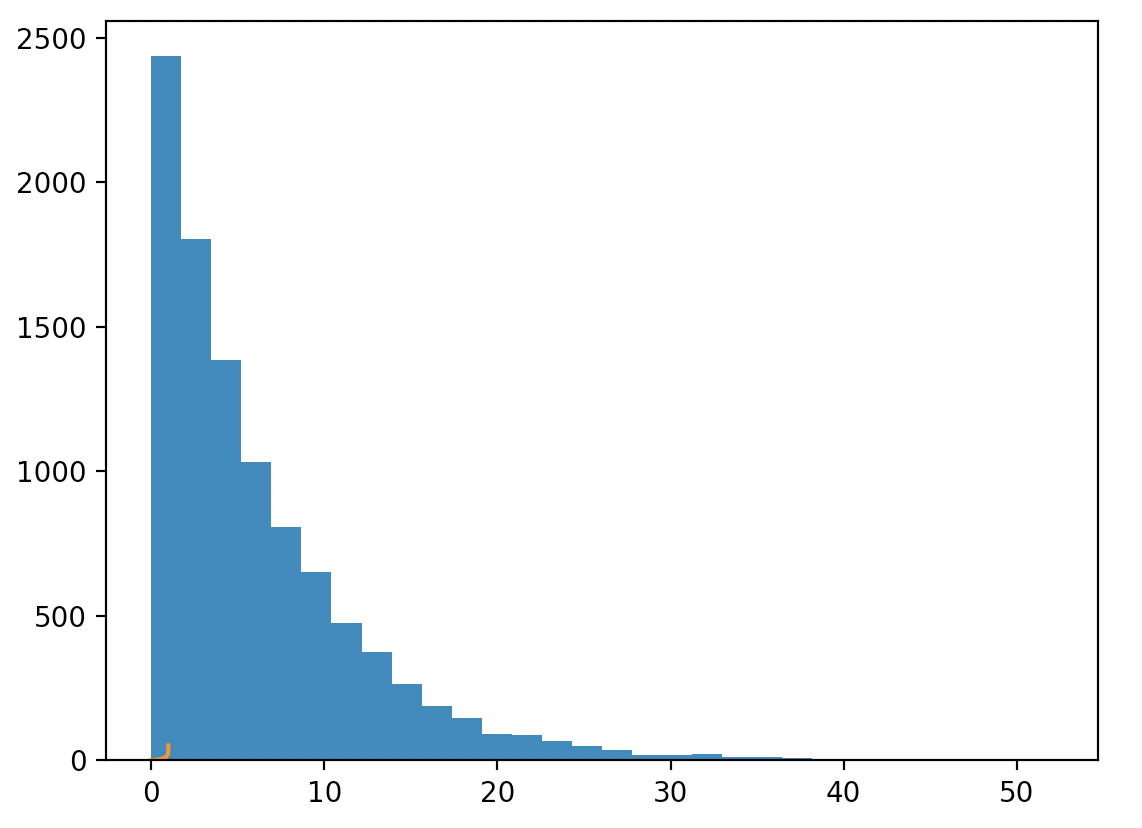
\includegraphics[scale=0.3]{{fig/exp_movie.png}}
    \caption{Exponential Distribution for Movie Votes}
\end{figure}

\subsection*{(c)}
\subsubsection*{airport: }
\begin{lstlisting}
    df = pd.read_csv("airport_routes.csv")
    print("a = ", df.min(), ", b = ", df.max())
\end{lstlisting}
Therefore, $[a,b] = [1,915]$.
\begin{figure}[H]
    \centering
    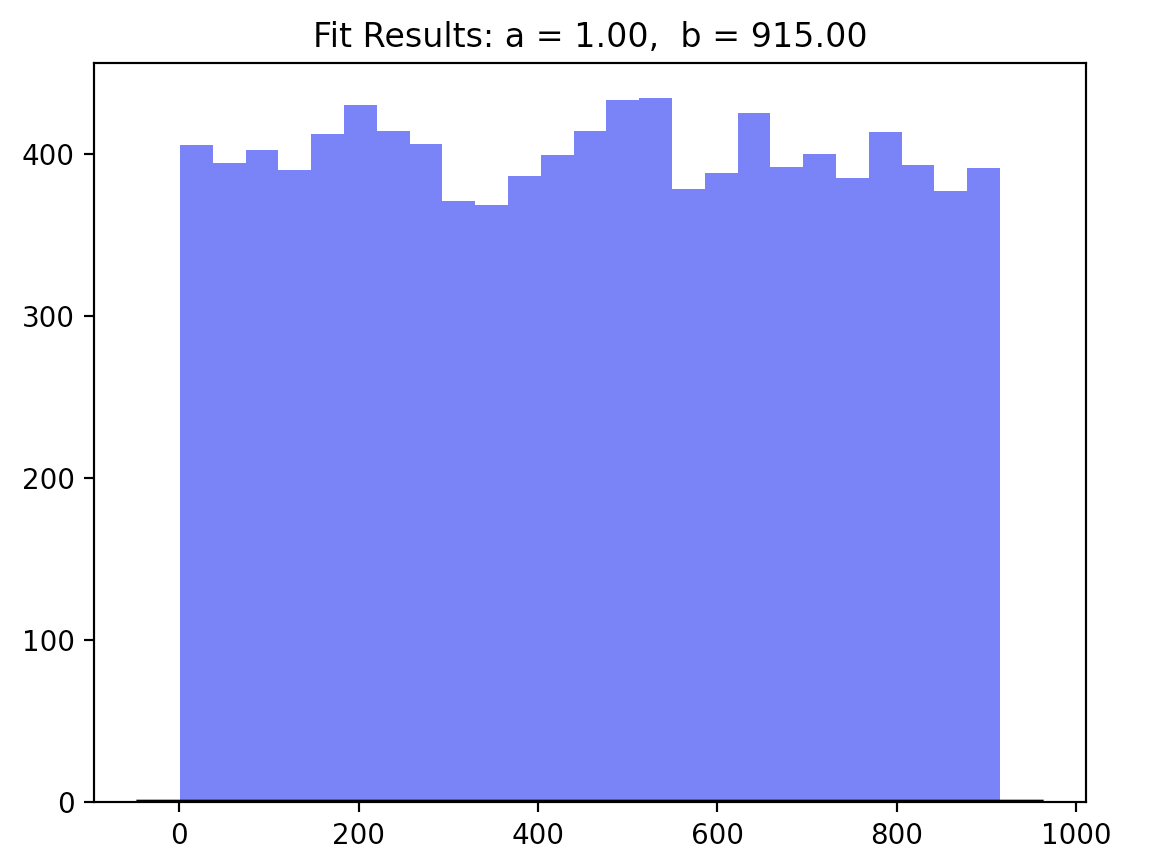
\includegraphics[scale=0.3]{{fig/uni_air.png}}
    \caption{Uniform Distribution for Airport Routes}
\end{figure}

\subsubsection*{movie: }
\begin{lstlisting}
    df = pd.read_csv("movie_votes.csv")
    print("a = ", df.min(), ", b = ", df.max())
\end{lstlisting}
Therefore, $[a,b] = [1.9, 8.5]$.
\begin{figure}[H]
    \centering
    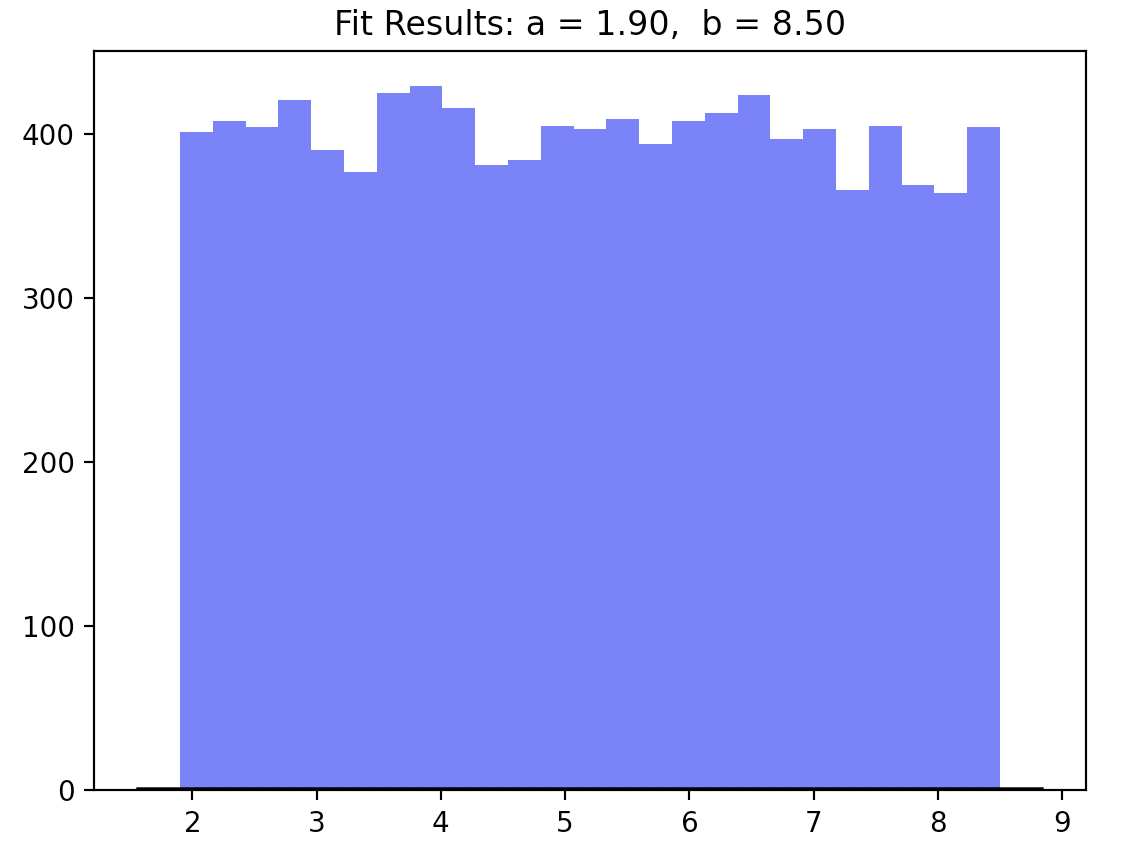
\includegraphics[scale=0.3]{{fig/uni_movie.png}}
    \caption{Uniform Distribution for Movie Ratings}
\end{figure}

\subsection*{(d)}
\subsubsection*{airport: }
\begin{lstlisting}
    df = pd.read_csv("airport_routes.csv")
    mean = df.mean(axis=0)
    std = df.std(axis=0)
\end{lstlisting}
Therefore, ($\mu$, $\sigma$) = (19.845116, 53.506467).
\begin{figure}[H]
    \centering
    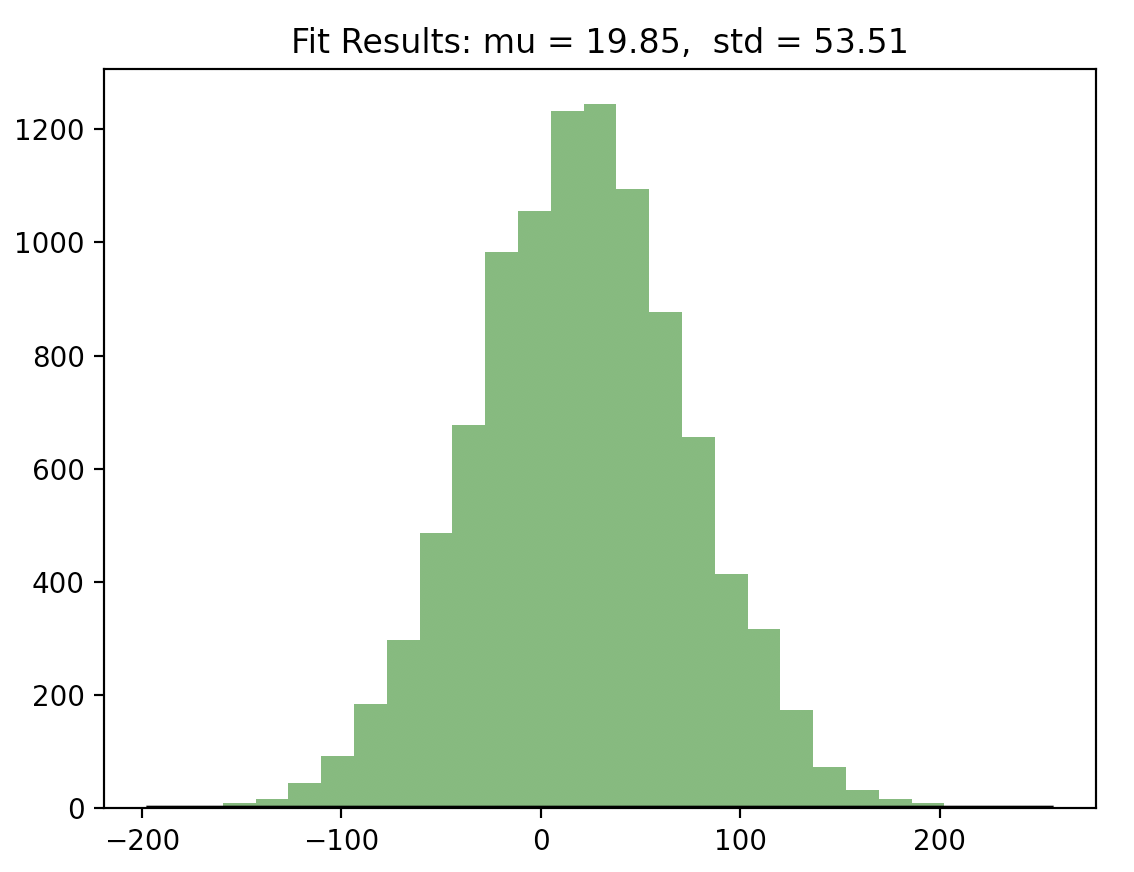
\includegraphics[scale=0.3]{{fig/norm_air.png}}
    \caption{Normal Distribution for Airport Routes}

\end{figure}

\subsubsection*{movie: }
\begin{lstlisting}
    df = pd.read_csv("movie_votes.csv")
    mean = df.mean(axis=0)
    std = df.std(axis=0)
\end{lstlisting}
Therefore, ($\mu$, $\sigma$) = (6.226935, 0.893215).

\begin{figure}[H]
    \centering
    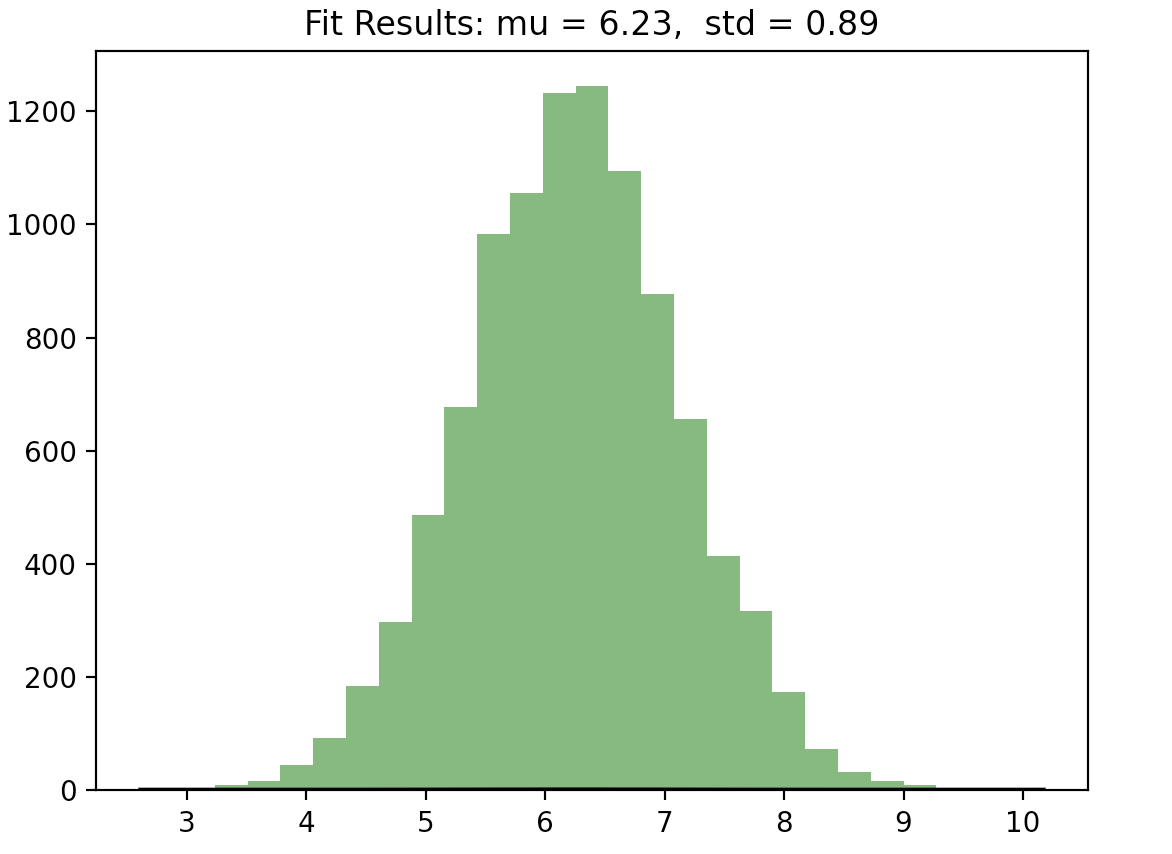
\includegraphics[scale=0.3]{{fig/norm_movie.png}}
    \caption{Normal Distribution for Movie Ratings}

\end{figure}

\subsection*{Analysis:}
The actual histogram plot for airport routes is:
\begin{figure}[H]
    \centering
    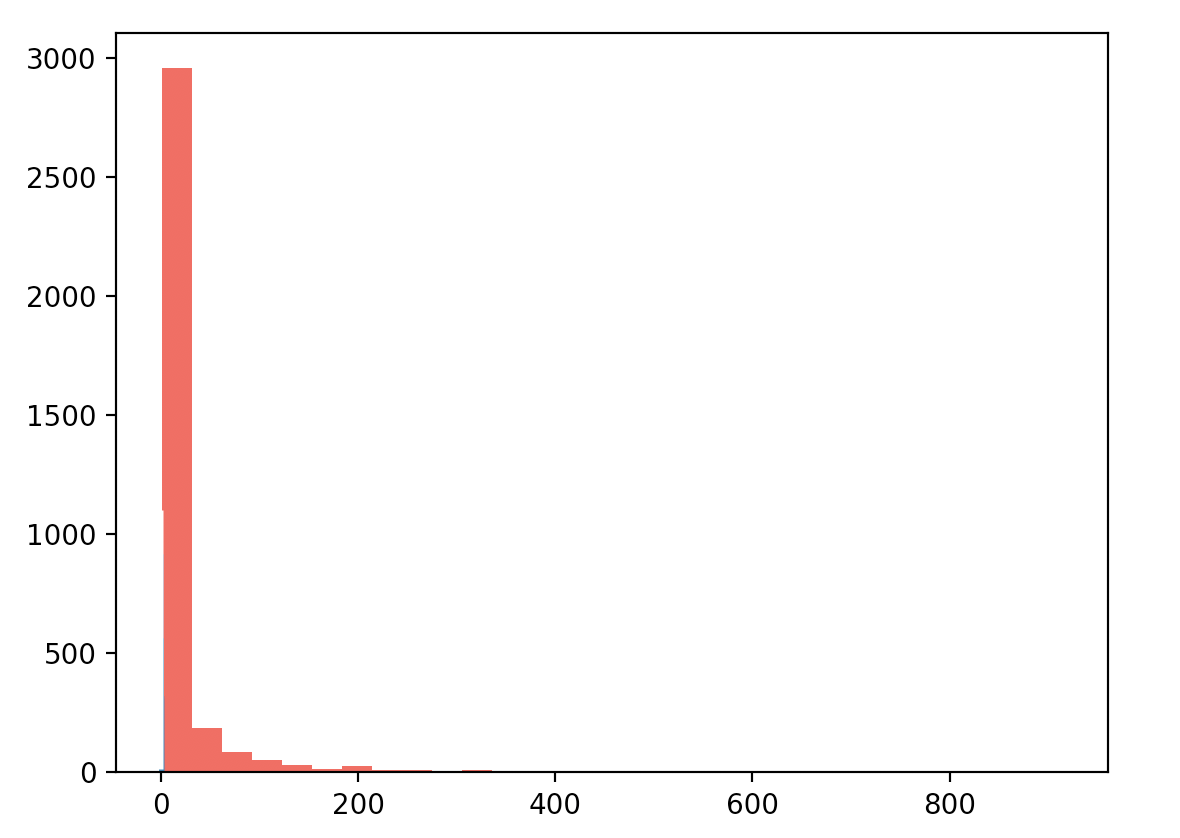
\includegraphics[scale=0.3]{{fig/data_air.png}}
    \caption{Actual Histogram for Airport Routes}

\end{figure}
We can tell it fits the exponential distribution the most according to its shape. Also, exponential distribution seems to be
a reasonable simulation since only a few of airports have a huge number of routes. Most of airports aggregate on the side with
relatively small number of routes. \\
The actual histogram plot for movie votes is:
\begin{figure}[H]
    \centering
    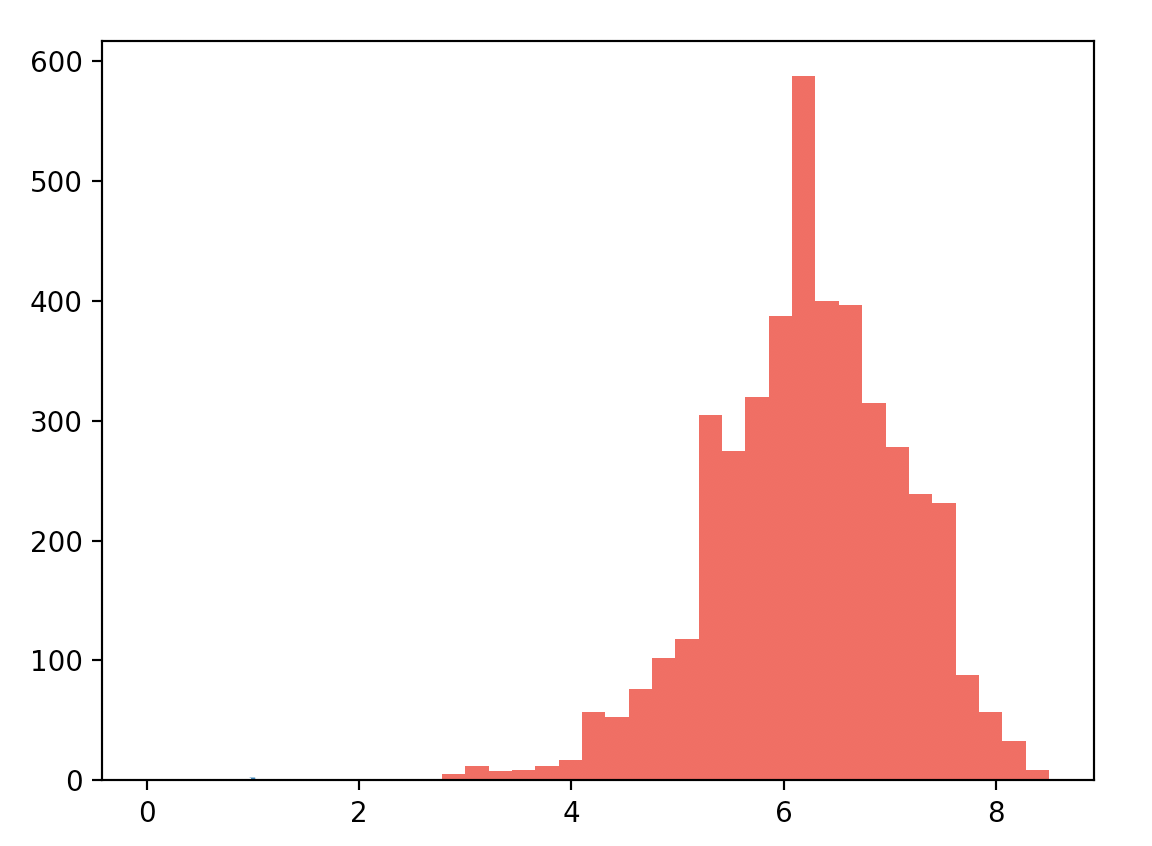
\includegraphics[scale=0.3]{{fig/data_movie.png}}
    \caption{Actual Histogram for Movie Ratings}

\end{figure}
We can tell it fits the normal distribution the most since the histogram seems to have a bell shape. The threshold appears around 6,
which agrees with the statistic we calculated before(around 6.22).



\section*{Problem 3}

\subsection*{(i)}

\begin{figure}[H]
    \centering
    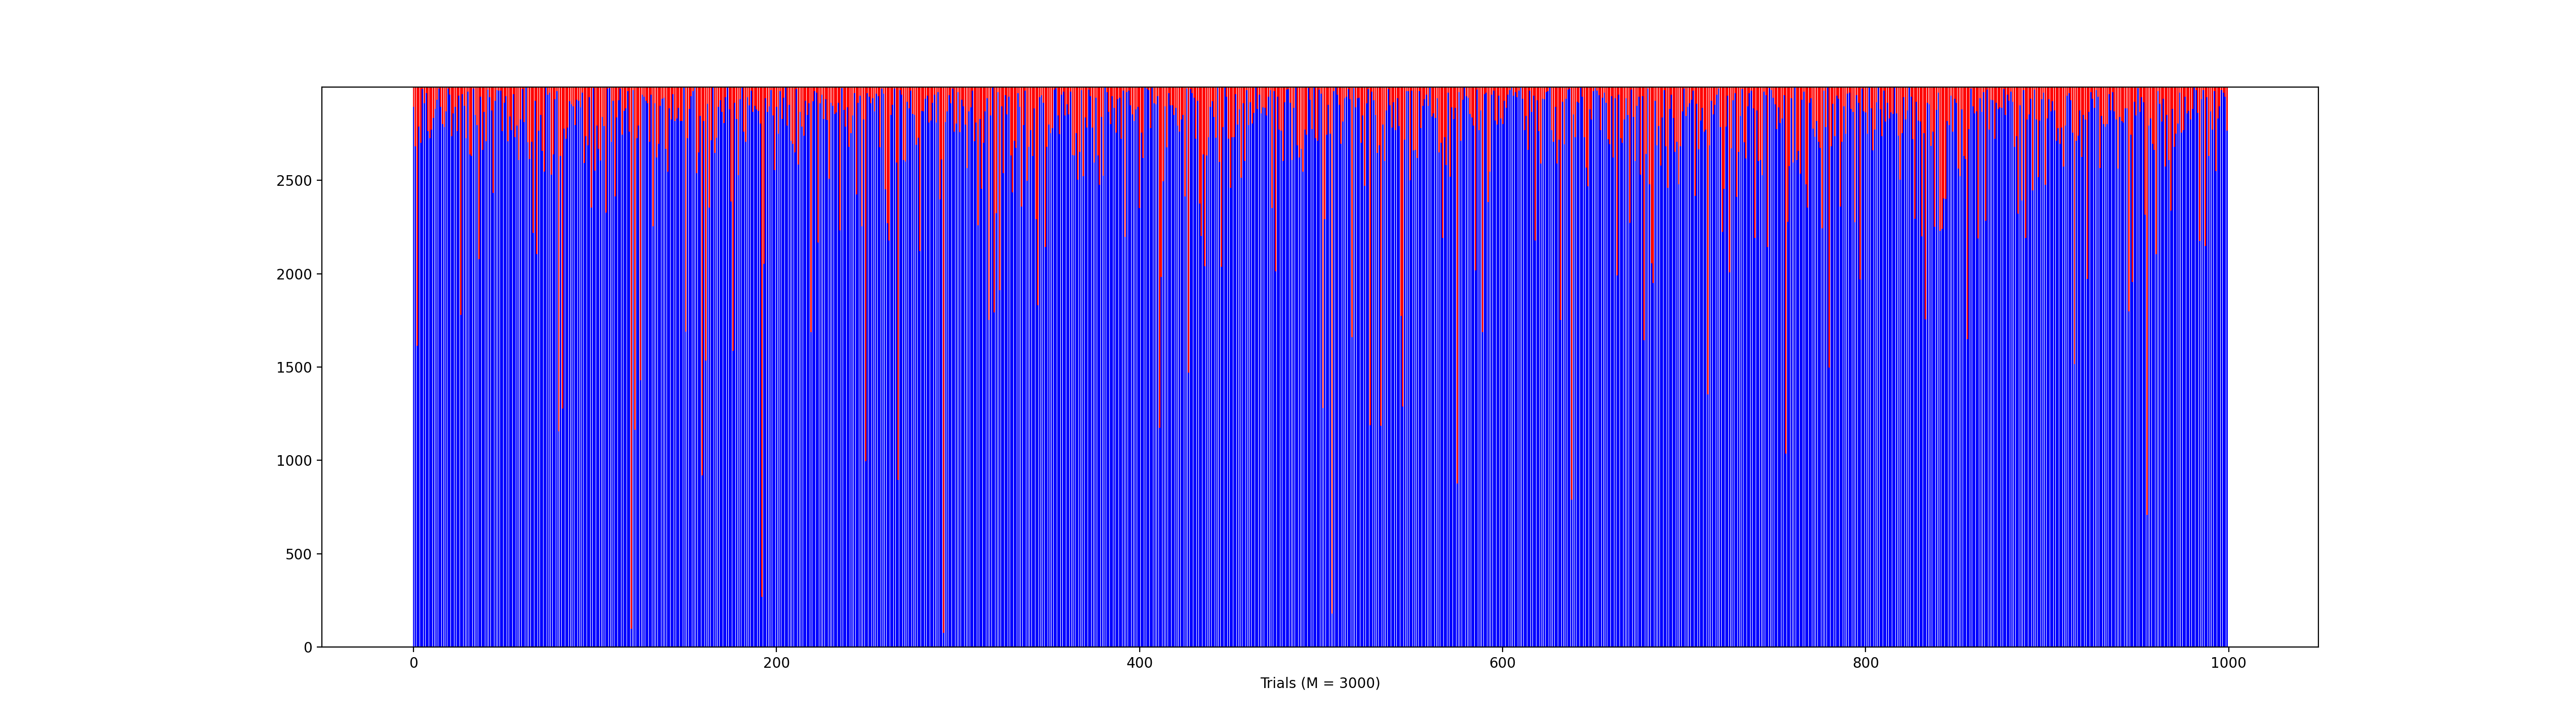
\includegraphics[width=1\linewidth]{{fig/fig_p3_1.png}}
    \caption{\textcolor{blue}{$E(MLE_M)$} v. \textcolor{red}{$E((M))$}}
\end{figure}

Note the \textit{MLE} for the population is just $M$ itself, thus $E(M) = M$. We simulated \ilc{1000} trials with $M = 3000$, where \textcolor{blue}{$E(MLE_M)$} is in blue, and its distance to \textcolor{red}{$E((M))$} is in red.

Note most of the trials there is a noticiable red bar between them, which shows the $M_{MLE}$ on sample is not an unbiased estimator of $M$.

\subsection*{(ii)}



$M_{MVU}$ showed a lower variance over our \ilc{1000} trials simulation. The average findings are below:

\begin{itemize}
    \item $Var(M_{MEAN})$: \ilc{2000277.10133029}
    \item $Var(M_{MVU})$: \ilc{2854104731.1510997}
\end{itemize}

We also picked \ilc{20} trials to visualize, not there the difference of the two estimators' variances are huge, as we can't even see the variance of $M_{MVU}$ without some extreme zooming.

\begin{figure}[H]
    \centering
    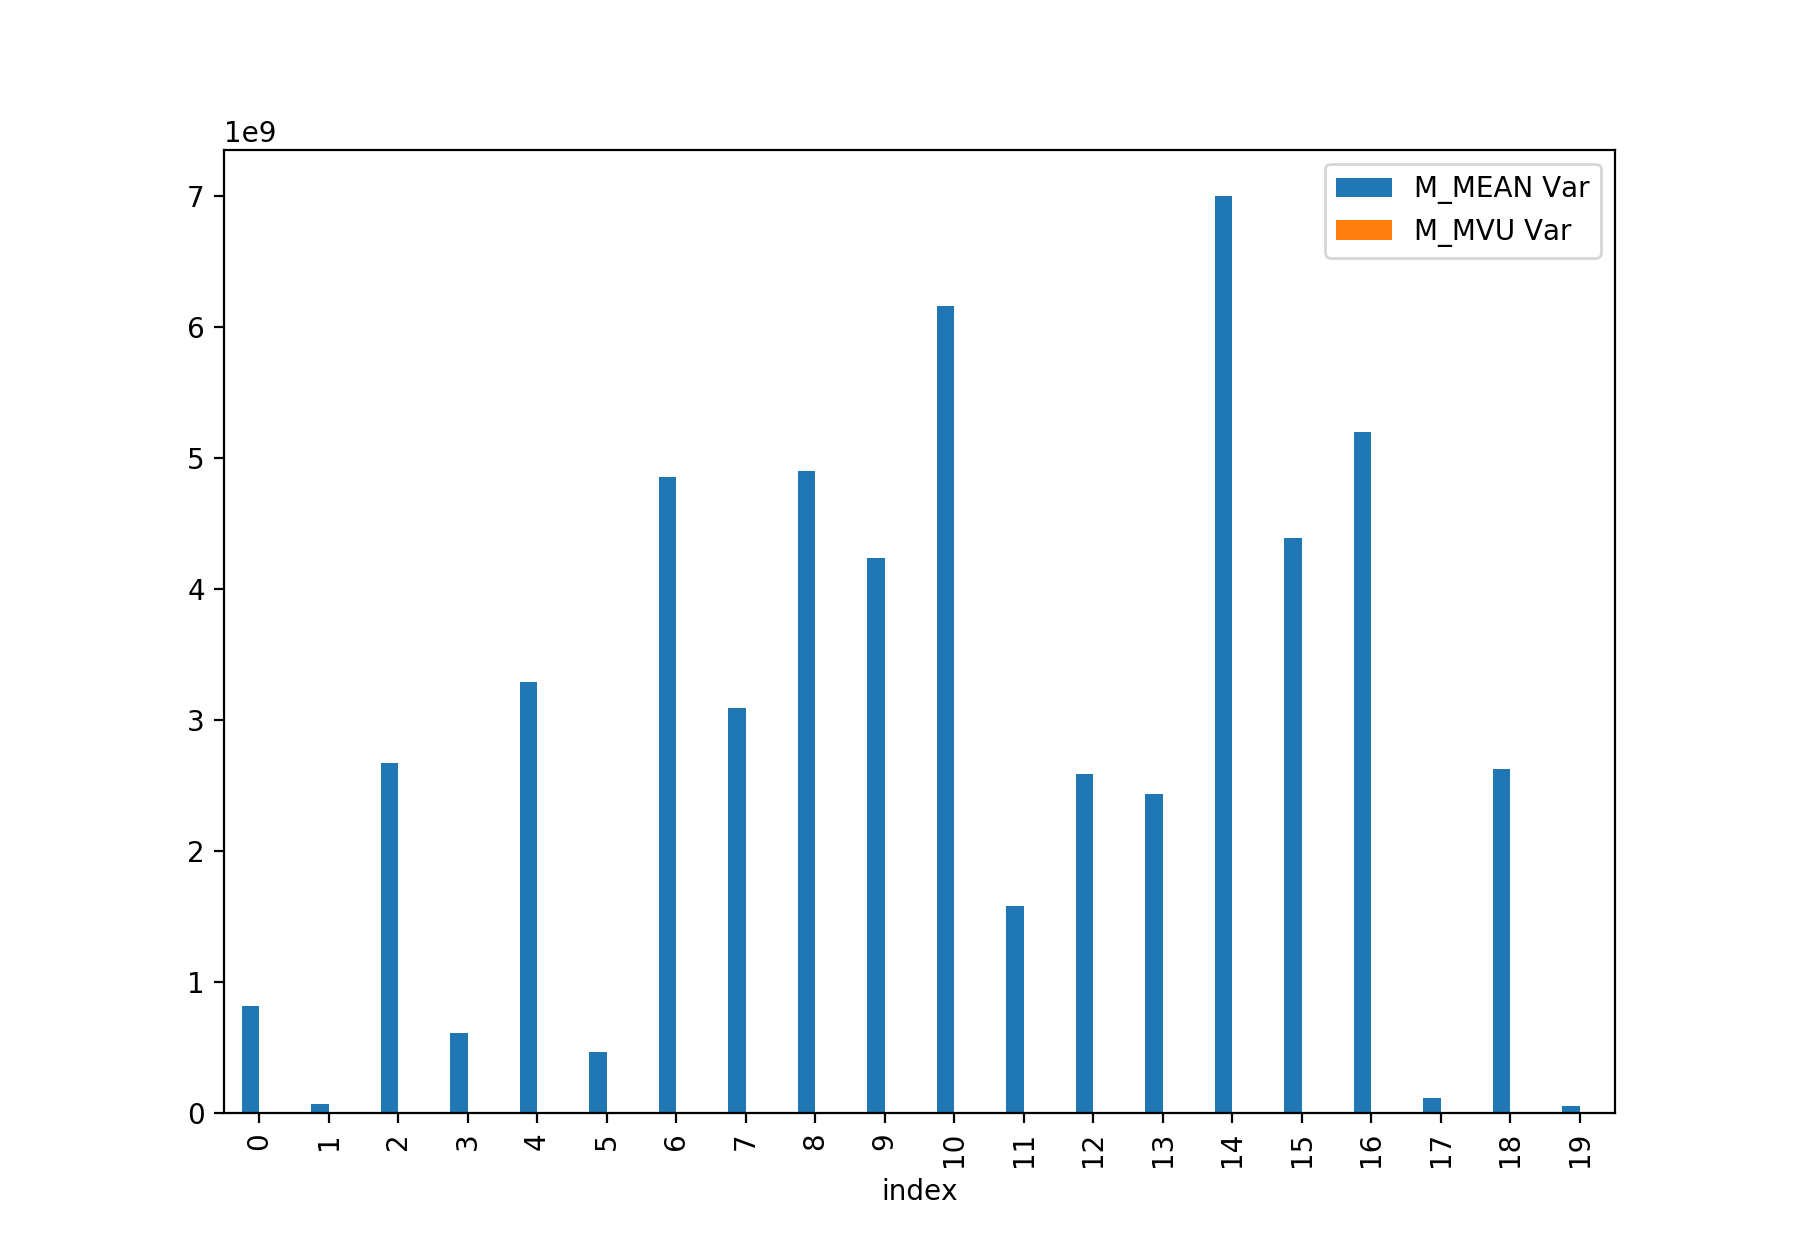
\includegraphics[width=0.5\linewidth]{{fig/fig_p3_2.png}}
    \caption{\textcolor{blue}{$Var(M_{MEAN})$} v. \textcolor{orange}{$Var(M_{MVU})$}}
\end{figure}


\end{document}